% -------------------------------------------------------------------------------- %

\begin{exercise}[Confidence interval 3]

Use \texttt R to generate a random sample $X_1, \dots, X_n$ from $\mathit{Pois}(1)$ distribution (for $n = 30$ and $n = 100$).
Compute the $90 \%$ confidence interval for $\lambda$, check if it contains the true value of $\lambda = 1$, and repeat ths $10 000$ times.
What is the fraction of simulations for which the confidence interval covers $\lambda$?

\end{exercise}

% -------------------------------------------------------------------------------- %

\begin{solution}

\phantom{}

\includepdf[
    pages = {9},
    nup = 1x2
]
{../../../EStat_VO/Lecture Slides/Lecture 9.pdf}

\lstinputlisting{10.4.r}

\end{solution}

% -------------------------------------------------------------------------------- %
